\documentclass[conference]{IEEEtran}
\IEEEoverridecommandlockouts
% The preceding line is only needed to identify funding in the first footnote. If that is unneeded, please comment it out.
\usepackage{cite}
\usepackage{amsmath,amssymb,amsfonts}
\usepackage{algorithmic}
\usepackage{graphicx}
\usepackage{textcomp}
\usepackage{xcolor}
\usepackage{tabularx}
\usepackage{multirow}
\usepackage{graphics} % for pdf, bitmapped graphics files
\usepackage{subfig}
\usepackage{subcaption}
\usepackage{hyperref}
\usepackage{academicons}
\usepackage{xcolor}
\usepackage{listings}
\def\BibTeX{{\rm B\kern-.05em{\sc i\kern-.025em b}\kern-.08em
		T\kern-.1667em\lower.7ex\hbox{E}\kern-.125emX}}
% Gráficas en MATLAB
\usepackage{tikz, pgfplots}
% Color Enlace
\definecolor{colorEnlace}{RGB}{0, 0, 0}
\hypersetup{
	colorlinks=true,
	linkcolor=colorEnlace,
	citecolor=colorEnlace,
	urlcolor=colorEnlace,
	pdfauthor={Davis Bremdow Salazar Roa},
	pdftitle={Experiencia N°6 Controlador PD y PID}
}
\lstset{
	language=Matlab, % Define el lenguaje
	basicstyle=\ttfamily\small, % Tamaño de letra pequeño
	keywordstyle=\color{blue}, % Color de las palabras clave
	commentstyle=\color{green}, % Color de los comentarios
	stringstyle=\color{purple}, % Color de las cadenas de texto
	numbers=left, % Muestra los números de línea a la izquierda
	numberstyle=\tiny\color{gray}, % Estilo de los números de línea
	tabsize=1,
	stepnumber=1, % Muestra un número en cada línea
	breaklines=true, % Ajuste automático de línea
	frame=single, % Borde alrededor del código
	xleftmargin=0em, % Elimina el margen izquierdo
	framexleftmargin=0em % Elimina el espacio dentro del marco izquierdo
}
% Control 
\usepackage{amsmath}
\begin{document}
	
	\title{Experiencia N°6 - Controlador PD y PID}
	% Ing. Diego Darcy Arredondo Huarac
	\author{	
		\IEEEauthorblockN{Davis Bremdow Salazar Roa}
		\IEEEauthorblockA{Universidad Nacional de San Antonio Abad del Cusco}
		\textit{Escuela Profesional de Ingeniería Electrónica}\\
		\textit{Laboratorio de Control I}\\
		200353 \\\\
		Cusco, Perú
	}
	
	\maketitle
	
	\begin{abstract}
		PD and PID controllers improve system stability and performance using root locus analysis. The PD controller adds a zero to adjust transient response and enhance system stability by increasing damping. Meanwhile, the PID controller combines proportional, integral, and derivative actions, refining both transient and steady-state performance. By strategically placing poles and zeros on the root locus, these controllers achieve desired dynamics and optimize control systems.
	\end{abstract}
	
	\begin{IEEEkeywords}
		PD controller, PID controller, root locus, stability, transient response, damping, proportional control, integral control, derivative control, pole placement.
	\end{IEEEkeywords}
	
	\section{Introducción}
		El diseño de controladores PD (Proporcional-Derivativo) y PID (Proporcional-Integral-Derivativo) es fundamental en el ámbito del control de sistemas dinámicos, especialmente para sistemas subamortiguados. Estos sistemas suelen caracterizarse por oscilaciones no deseadas y un sobreimpulso elevado en la respuesta transitoria, lo que puede comprometer su estabilidad y desempeño general. Los controladores PD y PID ofrecen herramientas versátiles para ajustar las características dinámicas del sistema, permitiendo reducir significativamente el sobreimpulso mientras se mejora la estabilidad y el tiempo de asentamiento. Este enfoque se basa en el ajuste preciso de los parámetros del controlador para alcanzar un equilibrio óptimo entre rapidez de respuesta y amortiguación.
		
		En particular, el controlador PD agrega un término derivativo que incrementa el amortiguamiento del sistema, reduciendo las oscilaciones y el sobreimpulso. Por otro lado, el controlador PID, al incluir un término integral, permite corregir errores de estado estacionario mientras mejora la respuesta transitoria mediante el ajuste combinado de los términos proporcional, derivativo e integral. A través de técnicas como el lugar geométrico de las raíces y el diseño en el dominio de la frecuencia, se pueden posicionar estratégicamente los polos y ceros del sistema, logrando un desempeño dinámico más adecuado a los requisitos específicos de la aplicación. Este enfoque es ampliamente utilizado en ingeniería para aplicaciones que demandan alta precisión y estabilidad, como sistemas robóticos, control de procesos y vehículos autónomos.
	\section{Objetivos}
	
	\begin{itemize}
		\item Diseñar Controlador PD y PID usando el Lugar Geométrico de las Raíces (LGR).
		\item Implementar Controlador PD y PID usando el Lugar Geométrico de las Raíces (LGR).
		\item Reducir el sobrepico a la mitad de un sistema subamortiguado mediante el uso del controlador PD, PID y el lugar geométrico de las raíces.
	\end{itemize}
	
	\section{Usando el Lugar Geométrico de las Raíces diseñar Controlador PD y PID}
	
	El inicio de un controlador mediante el lugar geométrico de las raíces (LGR), parte la ubicación de los polos y ceros en el plano imaginario y su proyección o posible ubicación en relación a la variación de un parámetro variable (normalmente la ganancia), en primera instancia se busca que el LGR tenga incluida en su trayectoria el polo dominante o deseado mediante el cual sistema ajuste su comportamiento según lo requerido y para mover las raíces del sistema a tal punto, solo seria necesario modificar la ganancia del sistema u otro parámetro modificable, no obstante si el polo deseado no pertenece al LGR será necesario agregar un elemento adicional (caso del controlador PD y/O PID) a la planta no modificable del sistema y mediante el cual se transformará el comportamiento del sistema para que se adapte a las necesidades esperadas, de forma forma concentra dentro del espectro del laboratorio se busca reducir el sobreimpulso a la mitad.
	
	En base a la premisa definida \textbf{¿Cuales son los parámetros iniciales del sistema que se buscan reducir?}, estos parámetros del sistema se pueden obtener a partir de la función de transferencia del sistema a lazo abierto y el cual esta definido en \ref{eq:ft-planta}
	
	\begin{equation}
		H(s) = \frac{65}{s^2 + 2s + 65}
		\label{eq:ft-planta}
	\end{equation}
	
	De la función de transferencia en concreto del polo del sistema al compararla con una ecuación de segundo grado como se define en \cite{ogata2015}, se puede obtener el factor de amortiguamiento $\xi$, la frecuencia natural $\omega_n$ y lo relevante para este caso el calculo del sobre impulso el cual se determina mediante la ecuación \ref{eq:sobreimpulso} y el cual es el parámetro de relevancia debido al objetivo del laboratorio.
	
	\begin{equation}
		M_p = 100e^{\frac{-\pi \xi}{\sqrt{1-\xi^2}}} 
		\label{eq:sobreimpulso}
	\end{equation}
	
	Además de este parámetro a pesar de ser considerados como elementos de segundo plano conocer la frecuencia natural y el tiempo de establecimiento $T_s$ nos facilitará la estimación del nuevo tiempo de respuesta y la velocidad en el establecimiento del sistema de forma que ello facilite la ubicación de los ceros para establecer los polos deseados como dominantes.
	
	Inicialmente el sistema cuenta con los siguiente parámetros característicos:
	\begin{align}
		M_p = 67.523 (Sobreimpulso) \\
		\xi &= 0.124 \\
		\omega_n &= 8.0623 \\
		T_s &= 4s (Tiempo de establecimiento) \\
		\label{eq:ts-planta}
	\end{align}
	
	Una vez establecidos estos parámetros se puede iniciar con el análisis, pero \textbf{¿Qué es lo que se desea cambiar?}, de forma directa se busca \textbf{reducir el sobreimpulso} a la mitad, por lo tanto el nuevo $M_p = 33.7616$, lo cual nos podrá brindar un nuevo valor del $\xi$ (factor de amortiguamiento), sin embargo para la obtención los polos deseados según \ref{eq:polos-deseados} también es necesario el valor la frecuencia natural $\omega_n$, por lo cual se tendrá que definir un valor para el tiempo de establecimiento el cual debido al agregado de ceros deberá ser más pequeño que el $T_s$ inicial.
	
	\begin{equation}
		S_{1,2} = -\xi \omega_n \pm j\omega \sqrt{1-\xi^2}
		\label{eq:polos-deseados}
	\end{equation}
	
	Al definir el nuevo $T_s = 0.2$ los polos deseados se ubicaran en $-20 \pm j57.86$ como se define en \ref{eq:polos-dominantes}
	
	\begin{equation}
		s_{1,2} = -20 \pm j22.33 
		\label{eq:polos-dominantes}
	\end{equation}
	
	Obteniendo que los nuevos valores para $\xi = 0.3267$ y la frecuencia natural $\omega_n = 61.2233 [\frac{rad}{s}]$ lo cual tiene sentido debido a que el $T_s$ se vio reducido.	

	
	Además cabe resaltar que obtener el nuevo valor de $\xi$ se hizo uso de \ref{eq:factor-amortiguamiento}, la cual nos permite calcular tal valor mediante el nuevo porcentaje y/o sobreimpulso.
	
	\begin{equation}
		\xi = \frac{-\ln(\frac{M_p}{100})}{\sqrt{\ln(\frac{M_p}{100})^2 + \pi^2}}
		\label{eq:factor-amortiguamiento} 	
	\end{equation}
	
	No obstante aun queda la duda de \textbf{¿Como incluir el LGR para el análisis del controlador PD y PID}, este se añade al diseño para poder ver gráficamente el comportamiento del sistema y la posible ubicación de los polos mediante la variación de una ganancia, es en tal sentido que en la figura \ref{fig:lgr-planta}
	
	\begin{figure}[h]
		\centering
		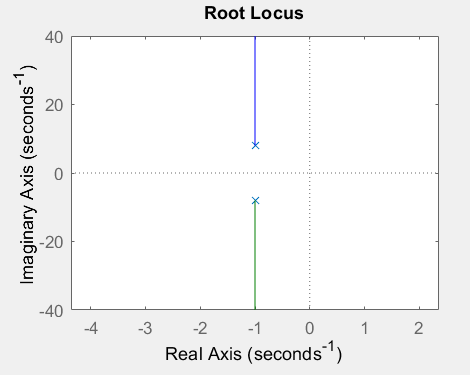
\includegraphics[width=0.5\textwidth]{media1/lgr-planta.png}
		\caption{Lugar geométrico del sistema a lazo abierto}
		\label{fig:lgr-planta}
	\end{figure}
	
	El criterio para el uso del control PID indica que el sistema se debe retroalimentar, aun así si bucle es unitario, por lo tanto para ver detalladamente el comportamiento de las raíces, analizar el LGR del sistema retroalimentado cuando $G_r(s) = 1$ nos puede brindar un mejor panorama del funcionamiento del sistema y donde se ubican las raíces en un lazo cerrado, este comportamiento se puede apreciar en la figura \ref{fig:lgr-planta-lc}
	
	\begin{figure}[h]
		\centering
		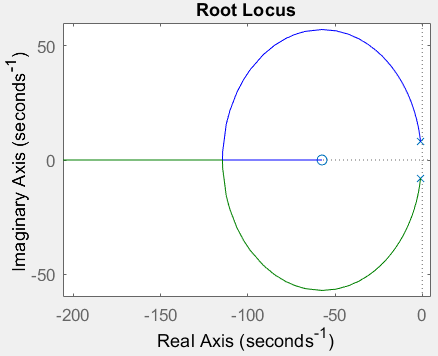
\includegraphics[width=0.5\textwidth]{media1/lgr-planta-lc}
		\caption{LGR del sistema a bucle cerrado cuando $G_r(s)$ = 1}
		\label{fig:lgr-planta-lc}
	\end{figure}
	
	Por otro lado en la parte matemática para el diseño del controlador PD y PID mediante el lugar geométrico, se hará uso de la condición de angulo y de magnitud para determinar el ángulo de compensación $\theta_m $ y la ganancia del sistema $k_a$.
	
	Para el cálculo de $\theta_m$ se hace uso de la ecuación \ref{eq:angulo-compensacion} el cual nos permitirá definir la contribución de angulo del controlador PD y/o PID para que el LGR pueda pasar por los polos deseados.
	
	\begin{equation}
		\sum<Z -\sum<P = -180
		\label{eq:angulo-compensacion}
	\end{equation}
	
	\subsection{Controlador PD}
	Haciendo uso de esta relación se puede apreciar que tal angulo de compensación $\theta_m = 36.95°$ y debido a la ubicación de este angulo que se encuentra definido en un triangulo rectángulo, el angulo $\theta_z$ será el complemento de este ángulo y con el cual mediante el calculo de la tangente se podrá calcular el valor del cero para el controlador PD.
	
	La distancia entre la parte real del polo deseado y la ubicación del cero en el eje real se puede obtener de la siguiente forma
	
	\begin{align}
		x &= \frac{57.86}{tg(53.05)} \\
		x &= 43.52 \\
		z &= 43.52 + 20 \\
		z &= 63.52 \\
		\label{eq:cero-pd-1}
	\end{align}
	
	Una vez determinado el cero del PD es posible calcular la ganancia del sistema mediante la condición de magnitud, la cual se define en \ref{eq:condicion-magnitud}
	
	\begin{equation}
		|G_c(s)G(s)| = 1
		\label{eq:condicion-magnitud}
	\end{equation}
	
	
	Obteniendo que el valor de la ganancia para el controlador PD será $k=0.77726$
	
	Finalmente el controlador PD tendrá la siguiente forma de \ref{eq:ft-pd}
	\begin{equation}
		G_r(s) = k(s + a)
		\label{eq:ft-pd}
	\end{equation}
	
	y estará matemáticamente definida como en \ref{eq:ft-pd-1}
	\begin{equation}
		G_r(s) = 0.77766(s + 63.52)
		\label{eq:ft-pd-1}
	\end{equation}
	
	\subsection{Controlador PID}
	El controlador PID definido matemáticamente en \ref{eq:ft-pid} a simple vista nos indica la existencia de un polo en el origen y ceros (no necesariamente conjugados), por lo tanto para aprovechar el potencial de este tipo de controlador que agregar un integrador (lo que facilita la sintonización) se definirán un polo en el origen y mediante el método de cancelación uno de sus ceros en la parte de real de las raíces de la función de transferencia siendo la otra calculada mediante el método usado para el controlador PD, obteniendo así que en angulo de compensación para este $\theta_m = 40.84°$ y la ganancia del sistema equivalente a $k_p = 0.7396$.
	\begin{equation}
		G_s(s) = k_p + \frac{T_i}{s} + T_ds
		\label{eq:ft-pid}
	\end{equation}
	
	Finalmente el controlador PID mediante el lugar de las raíces tendrá la forma de \ref{eq:ft-pid-1}
	\begin{equation}
		G_c(s) = \frac{0.7396(s + 1)(s + 70.01)}{s}
		\label{eq:ft-pid-1}
	\end{equation}
	
	\subsection{Adicionales}
	
	Finalmente como es común con los sistemas de control mediante PD o PID será necesaria ua sintonización de sus constantes, no obstante para el sistema propuesto no fue necesario una variación en la ganancia del sistema debido a que los parámetros iniciales calculados bastaron para poder cumplir con los requisitos deseados para el sistema.
	
	\section{Simulación del sistema de control en lazo cerrado diseñado mediante MATLAB}
	Una forma de poder comprobar los resultados obtenidos y que los controladores calculados son los adecuados es mediante el uso de MATLAB, siendo así que el código para el controlador PD, se tiene:
	\begin{lstlisting}[numbers=none, caption={Controlador PD}]
		clear, clc;
		% Planta del sistema
		num = [65];
		den = [1 2 65];
		
		planta = tf(num, den)
		
		% Raices del sistema a lazo abierto
		raicesPlanta = roots(den);
		disp("Raices Planta:"+raicesPlanta);
		
		wnInicial = sqrt(num(1));
		xiInicial = den(2)/(2*wnInicial);
		tsInicial = 4/(wnInicial*xiInicial);
		mpInicial = 100*exp(-pi*xiInicial/(sqrt(1 - xiInicial^2)) );
		fprintf("Parametros Iniciales");
		disp(["Freq. Natural Inicial: ", wnInicial]);
		disp(["Xi inicial: ", xiInicial]);
		disp(["Ts inicial: ", tsInicial]);
		disp(["Mp inicial: ", mpInicial]);
		
		fprintf("Nuevos parametros\n\n");
		% Parametros deseados
		mp = mpInicial/2; % sobreimpulso
		ts = 0.2; % sobreimpulso
		errorTs =  abs(tsInicial-ts)*100/tsInicial; % El porcentaje de error entre los Ts (inicial y experimental)
		disp(["Error en el Ts: ", errorTs+"%"]);
		% Calculo de los nuevos parametros
		xi = -log(mp/100)/( sqrt(log(mp/100)^2 + pi^2) );
		wn = 4/(xi*ts);
		disp(["Xi: ", num2str(xi)]);
		disp(["Mp deseado: ", mp]);
		disp(["Freq Natural: ", num2str(wn)]);
		
		% Calculo de los polos deseados
		pd = -xi*wn +i*wn*sqrt(1 - xi^2);
		disp(["Polo deseado: ", pd]);
		
		% Definiendo el Controlador PD
		zeroPD = [1 63.52];
		% Calculo de la ganancia
		ka = abs(evalfr(tf(den,zeroPD*num), pd));
		disp(["Ganancia PD: ", ka]);
		% Definiendo ganancia
		Gr = ka*zeroPD
		
		sistema = tf( 0.66*Gr*num , den )
		
		sistemaRetro = feedback(sistema,1)
		
		% Dibujando el LGR del sistema a lazo abierto
		figure(1); % Creando una figura
		subplot(2, 2, 1);
		rlocus(planta);
		subplot(2, 2, 2);
		rlocus(sistema);
		subplot(2, 2, 3);
		rlocus(sistemaRetro);
		% ================ PROBANDO EL SISTEMA ================
		figure(2); %
		tiempo_simulacion = 2;
		subplot(2, 1, 1);
		[resp_escalon_comp, t_escalon] = step(sistemaRetro, tiempo_simulacion);
		plot(t_escalon, resp_escalon_comp, 'b', 'DisplayName', 'Sistema Compensado');
		hold on;
		[resp_escalon_planta, t_escalon] = step(planta, tiempo_simulacion);
		plot(t_escalon, resp_escalon_planta, 'r', 'DisplayName', 'Planta');
		
		title('Respuesta al Escalon Unitario - Subamortiguado');		xlabel('Tiempo (s)');
		ylabel('Amplitud');
		legend show;
		grid on; 
		hold off;
		
		% Subgrafica 2: Respuesta al impulso 
		subplot(2, 1, 2); 
		[resp_impulso_comp, t_escalon] = impulse(sistemaRetro, tiempo_simulacion);
		plot(t_escalon, resp_impulso_comp, 'b', 'DisplayName', 'Sistema Compensado');
		hold on;
		[resp_impulso_planta, t_escalon] = impulse(planta, tiempo_simulacion);
		plot(t_escalon, resp_impulso_planta, 'r', 'DisplayName', 'Planta');
		
		title('Respuesta al Impulso Unitario  - Subamortiguado');
		xlabel('Tiempo (s)');
		ylabel('Amplitud'); 
		legend show;
		grid on; 
		hold off;
		sgtitle('Respuestas Sistema subamortiguado con Retroalimentacion Unitaria');
	\end{lstlisting}
	
	Para el caso del controlador PID la simulación en MATLAB se realizo mediante el entorno no gráfico y mediante el empleo del código en el cual se definieron las funciones de transferencia, compensadores y ganancias del sistema.
	
	\begin{lstlisting}[numbers=none, caption={Controlador PID}]
		clear, clc;
		% Planta del sistema
		num = [65];
		den = [1 2 65];
		
		planta = tf(num, den)
		
		% Raices del sistema a lazo abierto
		raicesPlanta = roots(den);
		disp("Raices Planta:"+raicesPlanta);
		
		wnInicial = sqrt(num(1));
		xiInicial = den(2)/(2*wnInicial);
		tsInicial = 4/(wnInicial*xiInicial);
		mpInicial = 100*exp(-pi*xiInicial/(sqrt(1 - xiInicial^2)) );
		fprintf("Parametros Iniciales\n\n");
		disp(["Freq. Natural Inicial: ", wnInicial]);
		disp(["Xi inicial: ", xiInicial]);
		disp(["Ts inicial: ", tsInicial]);
		disp(["Mp inicial: ", mpInicial]);
		
		fprintf("Nuevos parametros\n\n");
		% Parametros deseados
		mp = mpInicial/2; % sobreimpulso
		ts = 0.20; % sobreimpulso
		errorTs =  abs(tsInicial-ts)*100/tsInicial; % El porcentaje de error entre los Ts (inicial y experimental)
		disp(["Error en el Ts: ", errorTs+"%"]);
		% Calculo de los nuevos parametros
		xi = -log(mp/100)/( sqrt(log(mp/100)^2 + pi^2) );
		wn = 4/(xi*ts);
		disp(["Xi: ", num2str(xi)]);
		disp(["Mp deseado: ", mp]);
		disp(["Freq Natural: ", num2str(wn)]);
		
		
		% Calculo de los polos deseados
		pd = -xi*wn +i*wn*sqrt(1 - xi^2);
		disp(["Polo deseado: ", pd]);
		
		% Definiendo el Controlador PD
		zeroPID = [1 70.01];
		poloPID = [1 0];
		zeroPID1 = [1 1];
		
		gcZero = num*conv(zeroPID, zeroPID1);
		gcPolo = conv(poloPID, den);
		
		% Calculo de la ganancia
		ka = abs(evalfr(tf(gcPolo,gcZero), pd));
		disp(["Ganancia PID: ", ka]);
		
		% Definiendo ganancia
		
		sistema = tf(0.66*ka*gcZero, gcPolo )
		
		sistemaRetro = feedback(sistema,1)
		
		% Dibujando el LGR del sistema a lazo abierto
		figure(1); % Creando una figura
		subplot(2, 2, 1);
		rlocus(planta);
		subplot(2, 2, 2);
		rlocus(sistema);
		subplot(2, 2, 3);
		rlocus(sistemaRetro);
		% ================ PROBANDO EL SISTEMA ================
		figure(2); %
		tiempo_simulacion = 2;
		subplot(2, 1, 1);
		[resp_escalon_comp, t_escalon] = step(sistemaRetro, tiempo_simulacion);
		plot(t_escalon, resp_escalon_comp, 'b', 'DisplayName', 'Sistema Compensado');
		hold on;
		[resp_escalon_planta, t_escalon] = step(planta, tiempo_simulacion);
		plot(t_escalon, resp_escalon_planta, 'r', 'DisplayName', 'Planta');
		
		title('Respuesta al Escalon Unitario - Subamortiguado');
		xlabel('Tiempo (s)');
		ylabel('Amplitud');
		legend show;
		grid on; 
		hold off;
		
		% Subgrafica 2: Respuesta al impulso
		
		subplot(2, 1, 2); 
		[resp_impulso_comp, t_escalon] = impulse(sistemaRetro, tiempo_simulacion);
		plot(t_escalon, resp_impulso_comp, 'b', 'DisplayName', 'Sistema Compensado');
		hold on;
		[resp_impulso_planta, t_escalon] = impulse(planta, tiempo_simulacion);
		plot(t_escalon, resp_impulso_planta, 'r', 'DisplayName', 'Planta');
		
		title('Respuesta al Impulso Unitario  - Subamortiguado');
		xlabel('Tiempo (s)');
		ylabel('Amplitud'); 
		legend show;
		grid on; 
		hold off;
		sgtitle('Respuestas Sistema subamortiguado con Retroalimentacion Unitaria');
	\end{lstlisting}
	
	A forma de resume el código mostrado simula un sistema de control compensado para una planta subamortiguada mediante un controlador PD y PID, reduciendo el sobreimpulso inicial y mejorando el tiempo de establecimiento y el calcula los parámetros iniciales como la frecuencia natural, el factor de amortiguamiento y el sobreimpulso, y define nuevos parámetros deseados o requeridos para el sistema utilizando para ello el lugar geométrico de las raíces para ubicar polos deseados.
	
	\section{Mostrar las gráficas del ítem anterior, ¿Cuál es la explicación de estas graficas?}
	\subsection{Controlador PD}
	Como se puede apreciar en la figura \ref{fig:respuesta-sistema} se puede apreciar la respuesta del sistema frente a una excitación de entrada del tipo escalón e impulso unitario, 
	
	\begin{figure}[h]
		\centering
		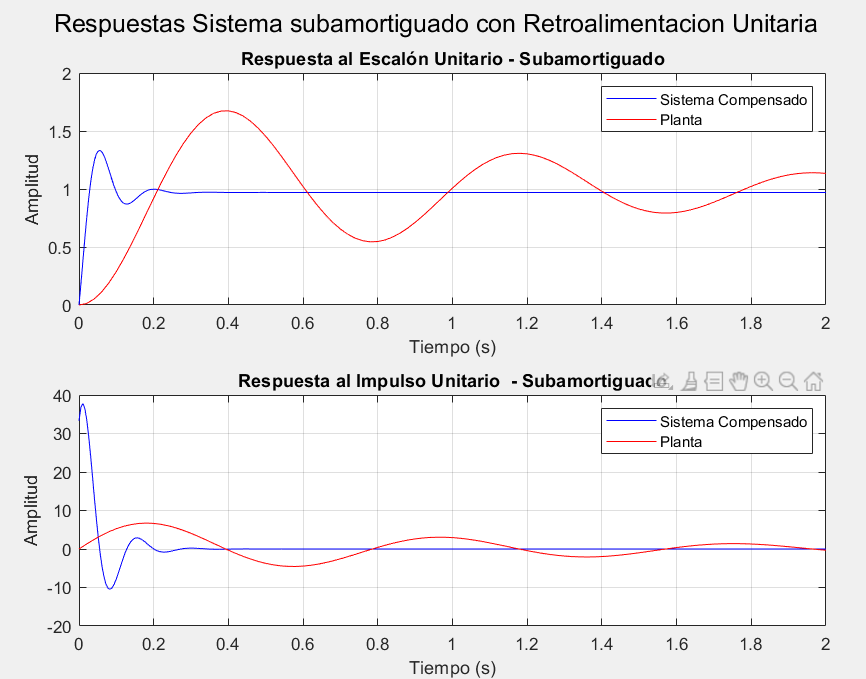
\includegraphics[width=0.5\textwidth]{media1/respuesta-sistema.png}
		\caption{Respuesta del sistema al escalón e impulso unitario - PD}
		\label{fig:respuesta-sistema}
	\end{figure}
	De la gráfica se puede apreciar que sistema original presenta un comportamiento subamortiguado típico, con oscilaciones iniciales notorias y un sobrepaso antes de estabilizarse y por otro lado el sistema original presenta un comportamiento subamortiguado típico, con oscilaciones iniciales notorias y un sobrepaso antes de estabilizarse y en la cual se puede apreciar una reducción el sobreimpulso y una aceleración en el tiempo de establecimiento.
	
	\subsection{Controlador PID}
	La respuesta del sistema mediante el controlador PID se muestra en \ref{fig:respuesta-sistema-pid} y en la cual se puede apreciar que al igual que el controlador PD se logra reducir el sobreimpulso, sin embargo en este caso la respuesta es menos brusca debido a los ceros que se agregaron y el polo en el origen que permite inestabilizar el sistema generando una mayor oscilación y un mayor tiempo de establecimiento.
	\begin{figure}[h]
		\centering
		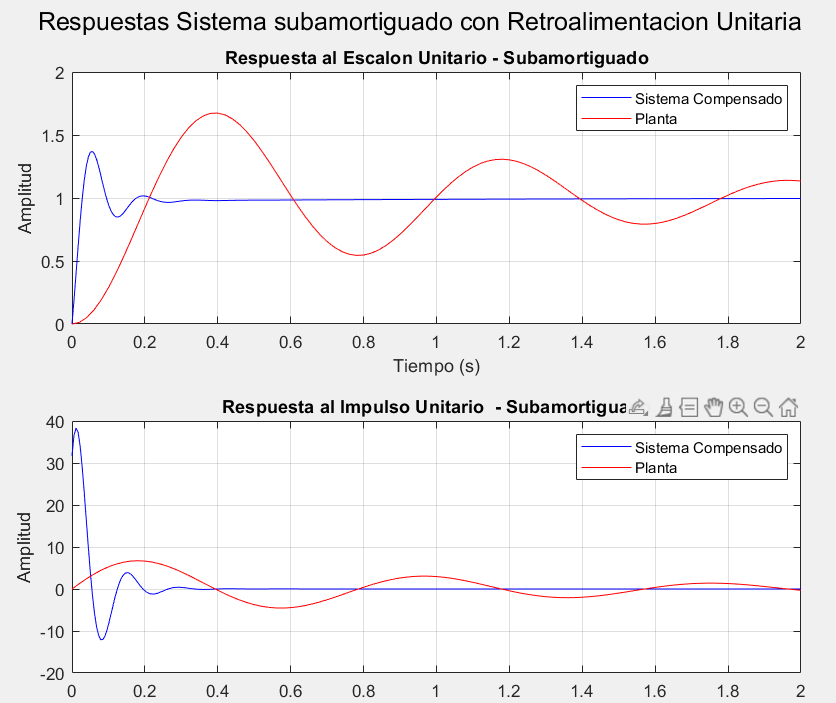
\includegraphics[width=0.5\textwidth]{media1/respuesta-sistema-pid.png}
		\caption{Respuesta del sistema al escalón e impulso unitario - PID}
		\label{fig:respuesta-sistema-pid}
	\end{figure}
	\bibliographystyle{IEEEtran}
	\bibliography{biblio}
\end{document}



































